% CREATED BY DAVID FRISK, 2016
\chapter{Sphere Tracing} \label{spheretracing}

	The graphics rendering algorithm our GPU was designed for is called Sphere
	Tracing\cite{Hart1996}. The name is based on the fact that the algorithm
	uses distance bounding spheres to incrementally advance along a ray in 3D space.
	The method of advancing along rays in general is called Ray Marching which in
	turn is a subset of Ray Tracing\cite{Whitted1980a}. Ray Tracing, is a
	way to wholly or partially render the world through rays, cast from the eye
	of the observer into the scene\cite{PeterShirleyMichaelAshikhmin2005}. 
	Sphere Tracing has been	around since at least as early as the late 
	eighties\cite{Hart1989} and Ray Tracing the 
	sixties\cite{Appel1968}.

	In this chapter the Sphere Tracing algorithm is discussed in detail with
	both definitions and examples. The explanation is based on the the very
	succinct explanation in \cite{Korndorfer2014}. The paper also expands upon
	the original algorithm in some innovative ways. For a more in-depth
	description of the original algorithm see Hart \cite{Hart1996}.

	\section{Sphere Tracing} 

		\begin{figure}
			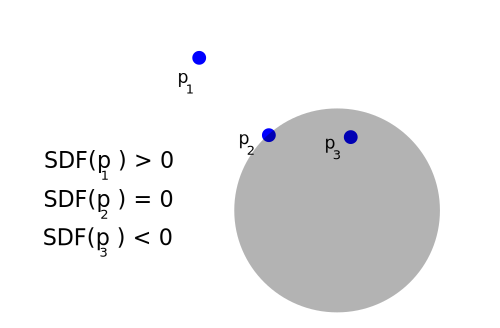
\includegraphics[width=0.75\linewidth]{figure/SDF} 
			\caption{Signed Distance Function of a sphere, sampled at three 
				points}
		\end{figure}

		The Sphere Tracing algorithm uses Signed Distance Functions to
		represent the geometry of a scene. If $f$ is a signed distance
		function: $$f : \mathbb{R}^{3}\mapsto\mathbb{R}$$ then $f$ returns, for
		all points in $\mathbb{R}^3$, the signed distance to the closest point
		on the implicit surface $\text{f}^{-1}(0)$. Signed in this context
		refers to the fact that the distance should be negative when measured
		on the inside of the surface.

		A common example would be the signed distance function, $f$, of a
		sphere centered at the origin with a radius of one: $f(\vec{v}) =
		|\vec{v}| - 1$. We can here see that a point $\vec{v}$ exactly on the
		surface would evaluate to $1-1=0$, any point outside of the sphere
		would evaluate to some positive distance and any point inside the
		sphere will result in a negative distance. It is, as will be discussed
		later, possible to generalize these distance functions to both unsigned
		distance functions and different kinds of distance bounds and
		approximations.

		If we define a ray $r(s) = \vec{d} \cdot s + \vec{o}$ where $\vec{d}$
		is the direction of the ray and $\vec{o}$ the origin, then $f\circ r(s)
		= 0$ means that the ray intersects the surface described by $f$ at
		exactly distance $s$ from the view point origin. Sampling every signed
		distance function in a given scene and returning the smallest value
		yields a function known as a distance field. Finding the surface can be
		done by marching point by point from the origin along the ray like
		below: 
		
		$$p_{i+1} = p_i + \vec{d}\cdot f(p_i)$$ 
		
		\begin{figure}
			\centering
			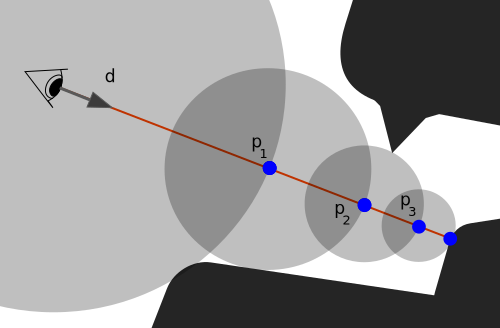
\includegraphics[width=0.75\linewidth]{figure/SDF2}
			\caption{Finding the intersection of an implicitly defined surface
				and a ray con be done by marching point by point from the 
				origin along the ray as show here.}
		\end{figure}

		This is repeated until $f(p_i) \leq \varepsilon$ for a given precision
		limit $\varepsilon$. $f(p_i)$ is the furthest possible march distance
		the ray can march while still not overshooting any potential surfaces
		at iteration $i$. The direction to the closest surface point is never
		known, thus $f(p_i)$ can be interpreted as a spherical bound, giving
		the algorithm it's name. The Sphere Trace is usually performed for each
		pixel of the screen, almost simulating the light rays entering the
		lens of an eye or camera in reverse.
		
		\subsection{Generalized Distance Functions}

			It is also possible to generalize signed distance functions into
			signed distance bounds: we define signed distance bounds such that
			if $f$ is the signed distance function for a given object, $g$ is a
			signed distance bound to the same object iff $\forall{} \vec{v}.
			|g(\vec{v})| \leq |f(\vec{v})|$. The Sphere Tracing algorithm
			continues to function correctly (\emph{That is, it will not march
			past any object without detecting it}) when signed distance
			functions are exchanged with signed distance bounds. The reason for
			this is simple: given a position $\vec{p}$, a Sphere Tracer using
			signed distance bounds will march forward $g(\vec{v})$ distance
			units, whereas a Sphere Tracer using signed distance functions will
			march forward at least as far or further, since $f(\vec{v}) \geq
			g(\vec{v})$.

			Using signed distance bounds, it is easy to construct complex
			objects from simple primitives using constructive solid geometry.
			That is, constructing new objects using unions, intersections, and
			complements: Let $f$ and $g$ be signed distance bounds of $a$ and
			$b$ respectivley. $\textrm{min}(g, f)$ is then a signed distance
			bound for the union of $a$ and $b$, $\textrm{max}(g, f)$ is a
			signed distance bound for the intersection of $a$ and $b$, and $-f$
			is a signed distance bound for the complementary shape of
			$a$\cite{Hart1996}. The union of signed distance bounds relates nicely
			to how Sphere Tracers handle multiple objects in scenes. By taking
			the minimum of all distance functions it is in effect taking the
			union of all ojects in the scene.

			Signed distance bounds for objects are not unique for a given
			object, and not all signed distance bounds are useful for Sphere
			Tracing. Indeed, $f(\vec{v}) = 0$ is a signed distance bound for
			every object that exists, but a Sphere Tracer would stop tracing
			immediately upon evaluating this function, and no useful object
			would be rendered. A Sphere Tracer can still work well though, as
			long as the distance bounds are 'close enough' to the signed
			distance function of the object they represent\cite{InigoQuilez}. Being
			close enough is a fuzzy constraint, but generally the length of the
			gradient should be as close to 1 as possible for good
			results\cite{Keinert}.

			It is of course possible to relax this concept further, and use
			distance approximation functions. These can still work together 
			with a Sphere Tracer if they are 'close enough' to the signed 
			distance function for the object they are meant to represent, but
			correctness can be harder to achieve. Distance approximation 
			functions allow significantly greater flexibility when designing 
			objects however, making it possible to add e.g. sinusoidal 
			deformations\cite{Quilez, Keinert}.

			Another relaxation that can be considered is using unsigned 
			distance functions. This might reduce the complexity of the 
			distance function, but it also reduces the stability of the Sphere
			Tracing algorithm and invalidates some optimizations that are 
			possible for their signed counterparts, such as predictive 
			overstepping\cite{Korndorfer2014}.

		\subsection{Reflections, refractions and shading}

			Once a point on a surface for a given pixel has been located,
			reflections, light, shadows and refractions needs to be calculated.
			A lot of these depend on the surface normal which can be
			approximated with the partial derivatives around the surface point
			given some small delta $\delta$. This is the normalized gradient
			$\vec{g}$ of the point.

			$$\vec{g} = \vec{x}\cdot\frac{\text{SDF}(x+\delta, y, z)}{\delta} +
			\vec{y}\cdot\frac{\text{SDF}(x, y+\delta, z)}{\delta} +
			\vec{z}\cdot\frac{\text{SDF}(x, y, z+\delta)}{\delta} $$

			$$\vec{n} = \frac{\vec{g}}{|\vec{g}|} $$

			A simple way to illuminate the scene could for an example be to use
			Phong Lightning\cite{Phong1975}. But any number of alternative
			algorithms could be used instead to determine the final color.
			Shadows can be determined by further Sphere Tracing out towards the
			sources of light from the surface to check for obstructions. Same for reflections
			and refractions where further marching in proportionate angles to
			the angle of incidence can determine what objects reflects on the
			surface.
